%%%%%%%%%%%%%%%%%%%%%%%%%%%%%%%%%%%%%%%%%12pt: grandezza carattere
%a4paper: formato a4
%openright: apre i capitoli a destra
%twoside: serve per fare un
%   documento fronteretro (oneside altrimenti)
%report: stile tesi (oppure book)
\documentclass[12pt,a4paper,openright,oneside]{report}
%
%%%%%%%%%%%%%%%%%%%%%%%%%%%%%%%%%%%%%%%%%libreria per scrivere in italiano
\usepackage[italian]{babel}
%%%%%%%%%%%%%%%%%%%%%%%%%%%%%%%%%%%%%%%%%libreria per accettare i caratteri
\usepackage[T1]{fontenc} 
\usepackage[utf8]{inputenc}
%
%%%%%%%%%%%%%%%%%%%%%%%%%%%%%%%%%%%%%%%%%libreria per impostare il documento
\usepackage{fancyhdr}
\usepackage{diagbox}
%
%%%%%%%%%%%%%%%%%%%%%%%%%%%%%%%%%%%%%%%%%libreria per avere l'indentazione
%%%%%%%%%%%%%%%%%%%%%%%%%%%%%%%%%%%%%%%%%   all'inizio dei capitoli, ...
\usepackage{indentfirst}
%
%%%%%%%%%%%%%%%%%%%%%%%%%%%%%%%%%%%%%%%%%libreria per inserire grafici
\usepackage{graphicx}
%
%%%%%%%%%%%%%%%%%%%%%%%%%%%%%%%%%%%%%%%%%libreria per utilizzare font
%   particolari ad esempio
%   \textsc{}
\usepackage{newlfont}
%
%%%%%%%%%%%%%%%%%%%%%%%%%%%%%%%%%%%%%%%%%libreria per tabelle multipagina
\usepackage{longtable}
%
%%%%%%%%%%%%%%%%%%%%%%%%%%%%%%%%%%%%%%%%%libreria per il rowspan e il colspan
\usepackage{multirow, multicol}
\newcommand{\sr}{\rule[-0.45cm]{0pt}{1.4cm}}
%
%%%%%%%%%%%%%%%%%%%%%%%%%%%%%%%%%%%%%%%%%libreria per tabelle multipagina
\usepackage[table]{xcolor}
%
%%%%%%%%%%%%%%%%%%%%%%%%%%%%%%%%%%%%%%%%%libreria per tabelle multipagina
%	con colonne centrate
\usepackage{array}
%
%%%%%%%%%%%%%%%%%%%%%%%%%%%%%%%%%%%%%%%%%libreria per produrre pagine landscape
%	in un documento principalmente portrait
\usepackage{pdflscape}
%
%%%%%%%%%%%%%%%%%%%%%%%%%%%%%%%%%%%%%%%%%libreria per l'inserimento di link nella
%   bibliografia
\PassOptionsToPackage{hyphens}{url}\usepackage[hidelinks]{hyperref}
%
%%%%%%%%%%%%%%%%%%%%%%%%%%%%%%%%%%%%%%%%%libreria per l'inserimento testuale
%	di frecce direzionali
\usepackage{textcomp}
%
%%%%%%%%%%%%%%%%%%%%%%%%%%%%%%%%%%%%%%%%%comando per l'inserimento di tab
\newcommand\tab[1][0,2cm]{\hspace*{#1}}
\newcommand\longtab[1][0,5cm]{\hspace*{#1}}
%
%%%%%%%%%%%%%%%%%%%%%%%%%%%%%%%%%%%%%%%%%comando per la gestione semplificata di quotes
\newcommand{\quotes}[1]{``#1''}
%%%%%%%%%%%%%%%%%%%%%%%%%%%%%%%%%%%%%%%%%comando per la gestione di legende a formule
\newenvironment{conditions}
{\par\vspace{\abovedisplayskip}\noindent\begin{tabular}{>{$}l<{$} @{${}={}$} l}}
	{\end{tabular}\par\vspace{\belowdisplayskip}}
%%%%%%%%%%%%%%%%%%%%%%%%%%%%%%%%%%%%%%%%%comando per il custom font size
\makeatletter
\newcommand{\codesize}{\@setfontsize{\srcsize}{7pt}{7pt}}
\makeatother
%
%%%%%%%%%%%%%%%%%%%%%%%%%%%%%%%%%%%%%%%%%librerie matematiche
\usepackage{amssymb}
\usepackage{amsmath}
\usepackage{latexsym}
\usepackage{amsthm}
%
%%%%%%%%%%%%%%%%%%%%%%%%%%%%%%%%%%%%%%%%%libreria per la visualizzazione di tree
\usepackage{dirtree}
%
%%%%%%%%%%%%%%%%%%%%%%%%%%%%%%%%%%%%%%%%%librerie per la visualizzazione del codice
\usepackage{listings}
\usepackage{color}
\definecolor{dkgreen}{rgb}{0,0.6,0}
\definecolor{gray}{rgb}{0.5,0.5,0.5}
\definecolor{redstrings}{rgb}{0.58,0,0.82}
\lstset{
	language=Java,
	captionpos=b,
	numbers=left,
	numberstyle=\tiny\color{gray},
	frame=tblr,
	tabsize=4, % tab space width
	showspaces=false,
	showtabs=false,
	breaklines=true,
	showstringspaces=false,
	breakatwhitespace=true,
	escapeinside={(*@}{@*)},
	basicstyle=\ttfamily\codesize,
	keywordstyle=\color{blue},
	commentstyle=\color{dkgreen},
	stringstyle=\color{redstrings}
}
%
%%%%%%%%%%%%%%%%%%%%%%%%%%%%%%%%%%%%%%%%%3d graph
\usepackage{pgfplots}
\usepackage{pgfplotstable}
\pgfplotsset{width=12cm,compat=1.8}
%
%%%%%%%%%%%%%%%%%%%%%%%%%%%%%%%%%%%%%%%%%multiline comments
\usepackage{verbatim} 
%
%%%%%%%%%%%%%%%%%%%%%%%%%%%%%%%%%%%%%%%%%impostazioni per il cambiamento di titolo
%	in lstlistoflistings
\renewcommand\lstlistingname{Codice}
\renewcommand\lstlistlistingname{Elenco dei codici}
\def\lstlistingautorefname{Codice}
%
\oddsidemargin=30pt \evensidemargin=20pt	%impostano i margini
\hyphenation{sil-la-ba-zio-ne thread}
%serve per la sillabazione: tra parentesi 
%vanno inserite come nell'esempio le parole 
%					   %che latex non riesce a tagliare nel modo giusto andando a capo.

%
%%%%%%%%%%%%%%%%%%%%%%%%%%%%%%%%%%%%%%%%%comandi per l'impostazione
%   della pagina, vedi il manuale
%   della libreria fancyhdr
%   per ulteriori delucidazioni
\pagestyle{fancy}\addtolength{\headwidth}{20pt}
\renewcommand{\chaptermark}[1]{\markboth{\thechapter.\ #1}{}}
\renewcommand{\sectionmark}[1]{\markright{\thesection \ #1}{}}
\rhead[\fancyplain{}{\bfseries\leftmark}]{\fancyplain{}{\bfseries\thepage}}
\cfoot{}
%%%%%%%%%%%%%%%%%%%%%%%%%%%%%%%%%%%%%%%%%
\linespread{1.3}                        %comando per impostare l'interlinea
%%%%%%%%%%%%%%%%%%%%%%%%%%%%%%%%%%%%%%%%%definisce nuovi comandi
%
\begin{document}
	\begin{titlepage}                       %crea un ambiente libero da vincoli
		%   di margini e grandezza caratteri:
		%   si pu\`o modificare quello che si
		%   vuole, tanto fuori da questo
		%   ambiente tutto viene ristabilito
		%
		\newpage                                %va in una pagina nuova
		%
		%%%%%%%%%%%%%%%%%%%%%%%%%%%%%%%%%%%%%%%%
		\clearpage{\pagestyle{empty}\cleardoublepage}%non numera l'ultima pagina sinistra
	\end{titlepage}
	\pagenumbering{roman}                   %serve per mettere i numeri romani
	\tableofcontents                        %crea l'indice
	%%%%%%%%%%%%%%%%%%%%%%%%%%%%%%%%%%%%%%%%%non numera l'ultima pagina sinistra
	\clearpage{\pagestyle{empty}\cleardoublepage}
	\listoffigures                          %crea l'elenco delle figure
	%%%%%%%%%%%%%%%%%%%%%%%%%%%%%%%%%%%%%%%%%non numera l'ultima pagina sinistra
	\clearpage{\pagestyle{empty}\cleardoublepage}
	\listoftables                           %crea l'elenco delle tabelle
	%%%%%%%%%%%%%%%%%%%%%%%%%%%%%%%%%%%%%%%%%non numera l'ultima pagina sinistra
	\clearpage{\pagestyle{empty}\cleardoublepage}
	\lstlistoflistings						%crea l'elenco dei codici+
	\pagenumbering{arabic}                  %mette i numeri arabi+
	%%%%%%%%%%%%%%%%%%%%%%%%%%%%%%%%%%%%%%%%%non numera l'ultima pagina sinistra
	\clearpage{\pagestyle{empty}\cleardoublepage}
	\chapter{Testo del progetto}           %crea il capitolo
	%%%%%%%%%%%%%%%%%%%%%%%%%%%%%%%%%%%%%%%%%imposta l'intestazione di pagina
	\lhead[\fancyplain{}{\bfseries\thepage}]{\fancyplain{}{\bfseries\rightmark}}
	\section{Specifiche}
	Dato il database relazionale Chinook e il relativo schema concettuale riportato
	in Figura \ref{fig:chinook_er}, si vogliono portare a termine i seguenti obiettivi.
	\begin{itemize}
		\item Progettazione concettuale di Schema di Fatto da schema E/R e relazionali.
		\item Analisi del carico di lavoro.
		\item Realizzazione di un cubo su Analysis Service.
		\item Preparazione di un report.
	\end{itemize}
	\section{Carico di lavoro}
	Il carico di lavoro complessivo è costituito da 4 query. Nelle seguenti sezioni si
	riportano sia quelle di natura obbligatoria per il gruppo in esame sia quelle aggiuntive
	relativamente il medesimo fatto di interesse.
	\subsection{Query di base}
	\begin{enumerate}
		\item Durata media delle tracce per artista.
		\item Numero di tracce per genere.
	\end{enumerate}
	\subsection{Query aggiuntive}
	\begin{enumerate}
		\item Dimensione media in byte delle tracce per genere.
		\item Durata media delle tracce per media type.
	\end{enumerate}
	\begin{figure}[!htb]
	\centering
	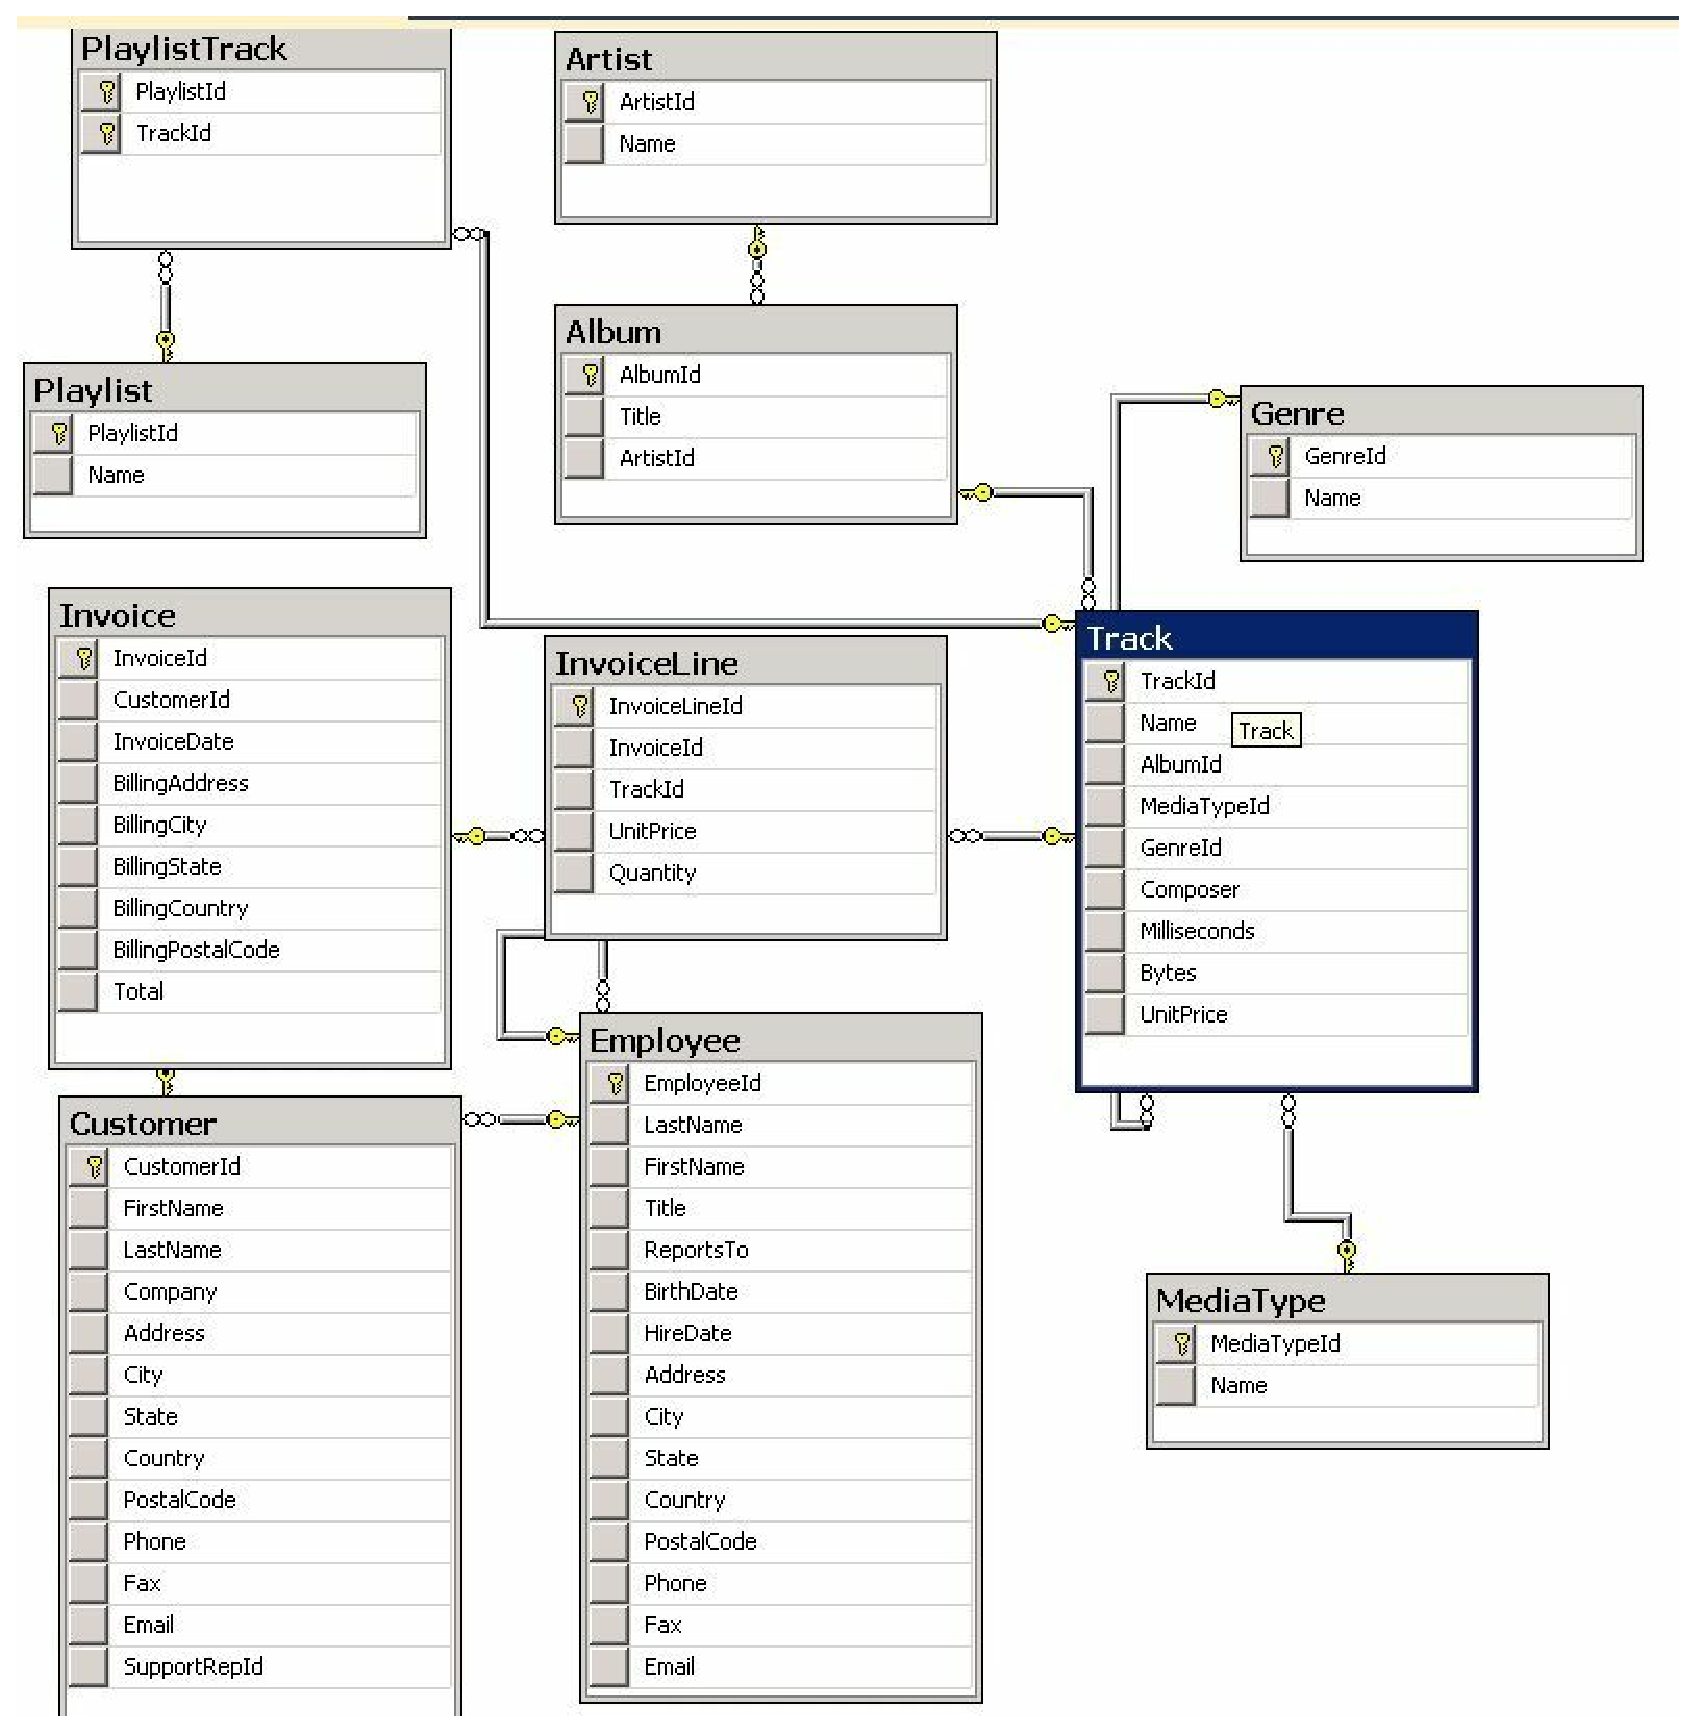
\includegraphics[scale=0.35]{eps/chinook_er.eps}
	\caption{Schema concettuale di Chinook}
	\label{fig:chinook_er}
	\end{figure}
	
	%%%%%%%%%%%%%%%%%%%%%%%%%%%%%%%%%%%%%%%%%non numera l'ultima pagina sinistra
	\clearpage{\pagestyle{empty}\cleardoublepage}
	\chapter{DFM}           %crea il capitolo
	%%%%%%%%%%%%%%%%%%%%%%%%%%%%%%%%%%%%%%%%%imposta l'intestazione di pagina
	\lhead[\fancyplain{}{\bfseries\thepage}]{\fancyplain{}{\bfseries\rightmark}}
	New chapter test.
	\section{Analisi del problema}						%crea la sezione
	Section test.
	
	\subsection{Requisiti}
	\label{subsec:GameOfLifeRequisiti}
	Nice subsection with \textit{Italic} test.
	\begin{quote}
		\textit{\quotes{Beautiful quoting}}
	\end{quote}
	An \emph{awesome} text.
	
	\subsection{Scelte intraprese}
	Subsection \#2, with new page.
	\newpage
	\section{Progettazione}						%crea la sezione
	Section \#3 with itemize:
	\begin{itemize}
		\item \textbf{1}, to do.
		\item \textbf{2}, to do.
	\end{itemize}
	
	\subsection{Dinamica del sistema}
	\label{subsec:GameOfLifeDinamica}
	Subsection with label.\\
	Figure citing \ref{fig:dinamica_gameoflife}.\\
	Equation:
	\begin{equation}
	N (compute) + N * (8 (ask neighbors) + 8 (neighbors reply) + 1 (notify grid))
	= 18N
	\label{eq:NumeroMessaggiSoluzioneSemplice}
	\end{equation}
	
	\subsection{GridActor}
	Example Code \ref{lst:gameoflife_gridactor} for file \textit{GridActor.java}.\\
	\begin{lstlisting}[caption=Classe GridActor - Game of Life, label=lst:gameoflife_gridactor]
	...
	
	/**
	* This actor represents a grid for the Conway's Game Of Life.
	* 
	*/
	public class GridActor extends AbstractActorWithStash {
	
	A beautiful class
	
	}
	\end{lstlisting}
	
	A table test.
	
	\begin{table}[h]
		\centering
		\begin{tabular}{ll|lllll|l}
			\cline{3-7}
			&                    & \multicolumn{5}{c|}{\textbf{Generazione}} &                            \\ \hline
			\multicolumn{1}{|l|}{\textbf{Modalità}}       & \textbf{Dimensione} & \textbf{5} & \textbf{10} & \textbf{20} & \textbf{50} & \textbf{100}   & \multicolumn{1}{l|}{\textbf{Media}} \\ \hline
			
			\multicolumn{1}{|l|}{\multirow{3}{*}{Attori}} & 100x100            & 26    & 21    & 18    & 16    & 16    & \multicolumn{1}{l|}{19,4}      \\ \cline{2-2} \cline{8-8} 
			\multicolumn{1}{|l|}{}                        & 500x500            & 1102  & 1077  & 1129  & 1293  & 1285  & \multicolumn{1}{l|}{1177,2}      \\ \cline{2-2} \cline{8-8} 
			\multicolumn{1}{|l|}{}                        & 1000x1000          & 20235 & 15724 & 14615 & 13949 & 13105 & \multicolumn{1}{l|}{15525,6}      \\ \hline
			\multicolumn{1}{|l|}{\multirow{3}{*}{Executor}} & 100x100            & 2     & 1     & 1     & 1     & 0     & \multicolumn{1}{l|}{1}      \\ \cline{2-2} \cline{8-8} 
			\multicolumn{1}{|l|}{}                        & 500x500            & 11    & 7     & 7     & 6     & 6     & \multicolumn{1}{l|}{7,4}      \\ \cline{2-2} \cline{8-8} 
			\multicolumn{1}{|l|}{}                        & 1000x1000          & 30    & 26    & 20    & 13    & 10    & \multicolumn{1}{l|}{19,8}      \\ \hline
		\end{tabular}
		\caption{Tempi di computazione alla n-esima generazione con differenti
			matrici di gioco a confronto coi risultati ottenuti nell'assignment \#1, in ms - Game of Life}
		\label{table:gameoflife_tempi_celle}
	\end{table}
	
	%%%%%%%%%%%%%%%%%%%%%%%%%%%%%%%%%%%%%%%%%non numera l'ultima pagina sinistra
	\clearpage{\pagestyle{empty}\cleardoublepage}
	\chapter{Schemi delle query su DFM}                %crea il capitolo
	%%%%%%%%%%%%%%%%%%%%%%%%%%%%%%%%%%%%%%%%%imposta l'intestazione di pagina
	\lhead[\fancyplain{}{\bfseries\thepage}]{\fancyplain{}{\bfseries\rightmark}}
	New chapter test.
	
	%%%%%%%%%%%%%%%%%%%%%%%%%%%%%%%%%%%%%%%%%non numera l'ultima pagina sinistra
	\clearpage{\pagestyle{empty}\cleardoublepage}
	\chapter{Schema logico}           %crea il capitolo
	%%%%%%%%%%%%%%%%%%%%%%%%%%%%%%%%%%%%%%%%%imposta l'intestazione di pagina
	\lhead[\fancyplain{}{\bfseries\thepage}]{\fancyplain{}{\bfseries\rightmark}}
	New chapter test.
	
	%%%%%%%%%%%%%%%%%%%%%%%%%%%%%%%%%%%%%%%%%non numera l'ultima pagina sinistra
	\clearpage{\pagestyle{empty}\cleardoublepage}
	\chapter{Report}           %crea il capitolo
	%%%%%%%%%%%%%%%%%%%%%%%%%%%%%%%%%%%%%%%%%imposta l'intestazione di pagina
	\lhead[\fancyplain{}{\bfseries\thepage}]{\fancyplain{}{\bfseries\rightmark}}
	New chapter test.
	
	
	%%%%%%%%%%%%%%%%%%%%%%%%%%%%%%%%%%%%%%%%%imposta l'intestazione di pagina
	\renewcommand{\chaptermark}[1]{\markright{\thechapter \ #1}{}}
	\lhead[\fancyplain{}{\bfseries\thepage}]{\fancyplain{}{\bfseries\rightmark}}
	\bibliography{relazione}
	\bibliographystyle{unsrt}
\end{document}